\subsection{Cpp2UML}

Afin d'avoir un rapide aperçu du projet ainsi qu'une vision globale des différentes classes réalisé et leurs dépendance,
nous avons tenté de générer un diagramme \textit{UML} de notre projet.

Un diagramme \textit{UML} est un façon de représenter le code de manière graphique.
Ce diagramme est composé d'une bulle, représentant une classe dans laquelle y est inscrit la liste des membres et attribut de cette classe avec des information de portée (privé, publique ...).
Chacune de ces bulles sont ensuite relié entre elles par différente flèche symbolisant les relation entre deux classe, on peut avoir des information filial, d'utilisation ou encore de contenance.

\begin{figure}[h!]
	\centering
	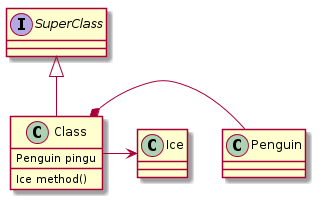
\includegraphics[width=0.8\textwidth]{img/uml_example.png}
	\caption{\textbf{Class} est une implementation d'une \textbf{SuperClass} qui utilise \textbf{Ice} et possède un \textbf{Penguin}, elle est composé d'un attribut \textit{pingu}, et d'une méthode \textit{surf}}
\end{figure}
\pagebreak
Dans le cadre de notre projet, nous avons réalisé un script en \textit{Lua},
permettant de générer automatiquement ce genre de graphique par le biais d'un autre outil:
\href{http://plantuml.sourceforge.net/}{PlantUML}.

Ce script annalyse les en tête de nos source afin d'écrire un autre fichier de description comprehensible par PlantUML. Une fois ceci fait, il ne reste qu'a lancer plantUML qui, en utilisant graphviz, crée une image, notre diagramme uml.
